% \begin{savequote}[8cm]
% Alles Gescheite ist schon gedacht worden.\\
% Man muss nur versuchen, es noch einmal zu denken.

% All intelligent thoughts have already been thought;\\
% what is necessary is only to try to think them again.
%   \qauthor{--- Johann Wolfgang von Goethe \cite{von_goethe_wilhelm_1829}}
% \end{savequote}

\chapter{\label{ch:studentuse}`Looking for Forests, Ignoring the Trees': Detecting and Monitoring Applicant AI Usage}

\minitoc

\section{Introduction}\label{sec:intro}
The powerful capabilities of modern generative AI challenge educators' ability to relate the quality of a student's writing to that student's talent. These challenges necessitate a change in the social structures designed to identify and measure talent. In particular, scholarship programs, universities, and other talent identification programs that rely on essays must reconsider how essays factor into the selection process. Such reconsideration may lead some programs to encourage AI-generated text so long as it is truthful and well-written, while others may ban the use of generative AI altogether. In the former case, it is useful to know where essays were written or augmented by AI, while in the latter case, it is essential. In either case, knowledge of \textit{how many} essays were written or augmented by AI is needed to determine the urgency of solving these problems.

Many solutions to the problem of generative AI detection exist already, but all have significant practical limitations. OpenAI shut down its own detection tool ``due to its low rate of accuracy''  and multiple experiments find automated post-processing can dramatically further reduce detectors' ability to identify AI-generated content  \cite{kalpesh_krishna_paraphrasing_2023,vinu_sankar_sadasivan_can_2023,kirchner_new_2023}. Other experiments combining disparate data sources suggest detectors disproportionately identify as AI-generated certain subgroups' genuinely human-written content \cite{liang_gpt_2023}. However, while detection solutions have been tested in concocted settings and shown to be both beatable and biased, there is limited public evidence evaluating their \textit{utility} in practice \cite{liang_gpt_2023,kalpesh_krishna_paraphrasing_2023}. We present a case study illustrating the potential utility and limitations of AI detection. 

In particular, our contributions are:

\begin{enumerate}
  \item We show that in the context of a specific talent identification program, identification of AI-generated content is hampered by false positives and heterogeneous biases across certain demographic subgroups. We conclude that said identifications should not be used in high-stakes decisions such as the disqualification of an applicant.
  \item We demonstrate sufficient statistical power for cohort-level analysis, and illustrate a one way that organisations can use AI detection technology to extract useful aggregate insights.
  \item We find potential for identification of AI-generated content as a decision aid in lower-stakes decision-making, such as directing selection attention towards specific applicants or evaluating the comparative value of different pipelines and outreach channels.
\end{enumerate}

\section{Related Works}\label{sec:rw}
Three bodies of work inform our research here. The first introduces new generative AI models or adapts existing models. The second introduces methods of detecting AI-generated text. The third consists of evaluations of detection methods applied to generative AI models.

Models such as GPT-3, GPT-4, and PaLM have quickly surpassed what was previously thought possible with a natural language model \cite{brown_language_2020,chowdhery_palm_2022,openai_gpt-4_2023}. While their ability to respond with natural language is impressive, their use in education raises questions of fairness and pedagogical integrity \cite{hu_challenges_2023}. 

In part due to these questions, there are many approaches to detecting AI usage, a vast majority of them commercial. Researchers have developed methods such as DetectGPT and stylometric detection, while commercial approaches include AI Writing Check, CatchGPT, Copyleaks, GPT Radar, GPTZero,  Turnitin, and Originality.ai \cite{mitchell_detectgpt_2023,kalpesh_krishna_paraphrasing_2023,tharindu_kumarage_stylometric_2023,gptzero_gptzero_2023,kirchner_new_2023}. Perhaps the most popular of these approaches is GPTZero's approach, based on `perplexity' and `burstiness' \cite{liang_gpt_2023,kalpesh_krishna_paraphrasing_2023}. GPTZero defines `perplexity' in relation to their own generative model – when scanning text, their generative model determines what the most likely next token is at each stage and compares this to the actual next token. `Burstiness', in contrast, is a document-level score of variation of sentence lengths and structures. The overall scores generated by GPTZero that we use are a combination of perplexity and burstiness \cite{gptzero_gptzero_2023}.

External evaluations of AI detectors represent a rapidly growing body of work. Some studies conclude that detection algorithms can be effective across a variety of simple tasks \cite{mitchell_detectgpt_2023,tharindu_kumarage_stylometric_2023,kalpesh_krishna_paraphrasing_2023}. Other evaluations find that under more complicated tasks, such as detecting paraphrased AI-generated text, these detectors perform less well \cite{kalpesh_krishna_paraphrasing_2023}. Separately, researchers are beginning to evaluate potential implications of using imperfect AI detectors. For example, comparing detectors' false positive rates for genuinely human-generated essays by from a US-based essay competition ($N = 88$) against those from Chinese English-language test takers ($N = 91$), \textcite{liang_gpt_2023} conclude AI detectors are biased against non-native English writers. Little has been done evaluating these detectors' using real data in a consistent educational context. To our knowledge, there are no longitudinal studies tackling these challenges.

\section{Data}\label{sec:experiments}
\subsection{Program Data}\label{ssec:setting}
We partner with an anonymous talent identification program that runs an application process to find promising young people from around the world. We use data from two of the program's application cycles, which we term Cycle 2022 and Cycle 2023.

Applications for Cycle 2022 were due in early 2022, well before ChatGPT's public release, so we assume that these submissions were written without the use of generative AI \cite{openai_gpt-4_2023}. Applications for Cycle 2023 were due in early 2023, so generative AI tools were widely available and AI detection tools were already emerging; we thus make no such assumption for these applications \cite{kirchner_new_2023,gptzero_gptzero_2023,liu_deid-gpt_2023}.

We note here that a number of avoidance detection strategies (e.g., paraphrasers) have been proven to severely hamper state-of-the-art detection  \cite{kalpesh_krishna_paraphrasing_2023}. However, as of the 2023 deadline, the efficacy of these detection avoidance strategies was not well-known, so we assume these strategies were not widely employed, and that our ability to differentiate between AI-generated and human-generated content in 2023 submissions mirrors our ability to differentiate between genuine 2022 submissions and known ChatGPT-generated responses to the Cycle 2022 essay prompts.

\begin{table}[tbh]
    \centering
    \caption{Text Essays Submitted by Demographic Group}
    \label{tab:demo_counts}
    \begin{tabular}{ l r r }
        \toprule
        Demographic Group & 2022 Essays & 2023 Essays \\
        \midrule
        Male & $6,475$  & $11,080$ \\
        Female & $8,710$  & $13,380$ \\
        Other & $176$ & $355$ \\
        \midrule
        Caribbean & $128$ & $75$ \\
        East/Southeast Asia & $1,332$ & $395$ \\
        Five Eyes & $522$ & $1,865$ \\
        Former Soviet Union & $85$ & $705$ \\
        Indian Subcontinent & $2,130$ & $2,560$\\
        Latin America & $709$ & $2,855$ \\
        Mid East/North Africa & $1,363$ & $4,100$ \\
        Sub-Saharan Africa & $8,972$& $8,375$\\
        Other Europe & $59$ & $560$ \\
        Pacific Islands & $5$& $0$ \\
        \midrule
        Total & $15,149$ & $24,815$ \\
        \bottomrule
    \end{tabular}
    % \begin{tablenotes}
    %     \small
    %     \item `Five Eyes' consists of Australia, Canada, New Zealand, the United Kingdom, and the United States.
    % \end{tablenotes}
\end{table}

Each applicant submitted essays in response to five prompts. These prompts are not described in more detail to preserve our partner organisation's anonymity. Applicants in both cycles considered provided information on their background, including gender identity and countries of citizenship. Applicants were asked their gender identity and given options including `male', `female', `non-binary', `other', and `prefer not to say'. The vast majority selected `male' or `female', so, in order to avoid spurious results from small samples, we group `non-binary' and `prefer not to say' under `other' for this analysis. Similarly, we group nationalities into larger regional categories with shared cultural heritages. These regional groupings are our own; we have opted not to share a list of countries at the program's request and therefore cannot share specific country-to-region codings (with the exception of the `Five Eyes' region, which consists of Australia, Canada, New Zealand, the United Kingdom, and the United States). Table \ref{tab:demo_counts} describes the analytic sample of essays by these demographic dimensions for each cycle. 

\subsection{Synthetic Data}\label{ssec:chatgpt}
To obtain a set of known AI-generated essays, we generate $5,002$ synthetic essays using OpenAI's ChatGPT API and Cycle 2022 prompts. These sit alongside our $15,149$ human-written, applicant-submitted Cycle 2022 essays and form our Cycle 2022 corpus. In contrast, our Cycle 2023 corpus consists entirely of applicant-submitted essays, though it is unknown how many of these are AI-generated. Our entire corpus is detailed in Table \ref{tab:cycle_counts} The prompts provided to ChatGPT and the model version used is available in the appendices, and more detail on the model itself can be found in \cite{brown_language_2020}.

\begin{table}[tbh]
    \centering
    \caption{Essays by Source}
    \label{tab:cycle_counts}
    \begin{tabular}{ l r }
        \toprule
        Source  & Essays \\
        \midrule
        Cycle 2022 Submissions (Assumed Not AI) & $15,149$ \\
        ChatGPT Responses to Cycle 2022 Prompts & $5,002$ \\
        Cycle 2023 Submissions (Potentially AI) & $24,815$ \\
        \bottomrule
    \end{tabular}
\end{table}

\subsection{AI Detection Scores}\label{ssec:gptzero}
A number of generative AI detection tools are publicly available \cite{mitchell_detectgpt_2023,gptzero_gptzero_2023}. Among them, GPTZero has emerged as a leading solution to the problem \cite{gptzero_gptzero_2023}. Between 2 March and 6 April, 2023, we fed each essay in our sample into GPTZero's API using the default settings. This yielded various statistics for each essay, but we are primarily interested in $completely\_generated\_prob$, which is an overall likelihood statistic. More detail on GPTZero can be found in \cite{gptzero_gptzero_2023}.

\section{Experiments}
\subsection{AI Detection in High-Stakes Decision-Making}\label{ssec:exp_accuracy}
Instrumentally, we consider several possible uses of $completely\_generated\_prob$. If a program wishes to disqualify applicants for their use of generative AI, they must first determine whether such disqualification is possible. Thus, we are interested in the viability of using $completely\_generated\_prob$ for the automated disqualification of AI-generated applications. To determine this, we set a threshold for the acceptable True Positive Rate (TPR) and False Positive Rate (FPR). Our partner program selects only $2\%$ of completed applications, so any threshold with a false positive rate of $0.02$ or more would risk rejecting as many qualified candidates on the basis of erroneous AI detection as were ultimately admitted. We deem this unacceptable, so we focus on performance at $FPR \leq 0.02$. Following a liberal criterion whereby at least 3 in 4 applicants submitting completely AI-generated content would be identified, we consider a TPR of at least $75\%$ sufficient \cite{Bradley_1978}.

\subsection{AI Detection in Aggregate Statistics}\label{ssec:exp_statistics}
Regardless of a talent identification program's attitude towards the use of generative AI, we are also interested in estimating the prevalence of AI-generated content using group-level statistics. Since applicants may have edited AI-generated content or combined it with language they drafted, we do not use a specific threshold to test for differences in the proportion identified as completely AI generated. Instead, we note here that the mean probability of an essay being AI-generated across a corpus is exactly the expected proportion of AI-generated content within that corpus. Thus, we may test for differences in prevalence by testing for differences in the mean $P(AI)$. 

We note first that, while we can be confident $completely\_generated\_prob$ is a likelihood estimator, we do not know whether this statistic is a probability estimator \cite{gptzero_gptzero_2023,Platt_2000}. That is, we do not know whether, in expectation, 5 in 10 essays with $completely\_generated\_prob = 0.50$ are in fact AI-generated. To determine this, we first plot a histogram and calibration curve of $completely\_generated\_prob$ values on our Cycle 2022 data (Figures \ref{fig:c2_hist} and \ref{fig:c2_calibration} respectively).

\begin{figure}[tbh]
    \centering
    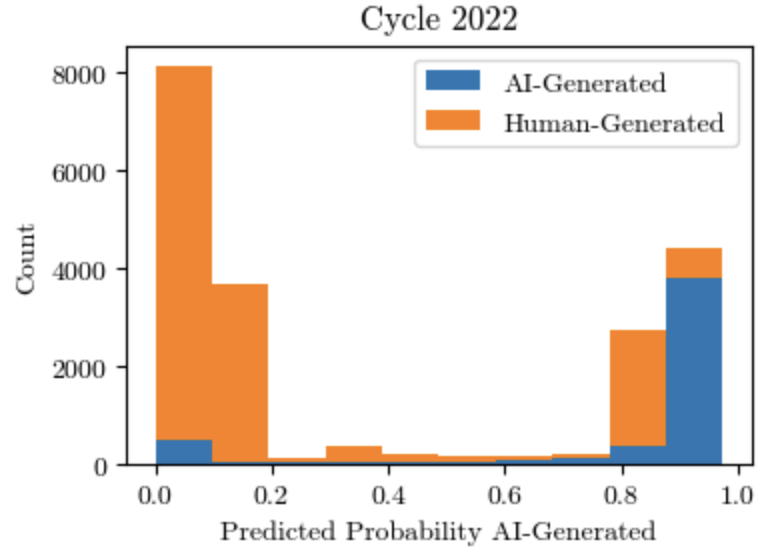
\includegraphics[width=0.4\textwidth]{figures/generative_ai/hist.png}
    \caption{Histogram of Uncalibrated GPTZero Scores, Cycle 2022}
    \label{fig:c2_hist}
\end{figure}

Figure \ref{fig:c2_hist} presents a histogram of uncalibrated GPTZero scores for the 2022 applicant-submitted and research-prompted, GPT-generated essays. Consistent with our knowledge that these essays were either entirely human-generated or entirely AI-generated, the histogram of values for $completely\_generated\_prob$ is bimodal. We see a large number of false positive essays with $completely\_generated\_prob \geq 0.8$. Similarly, Figure \ref{fig:c2_calibration} presents a calibration curve, which shows large differences between GPTZero's predicted probability and fraction of true positives in our data, proving that $completely\_generated\_prob$ is indeed not well-calibrated on our data. We thus perform statistic calibration on $completely\_generated\_prob$ to get an estimate of the probability that a given essay within our corpus is AI-generated (i.e., $\widehat{P(AI)}$) \cite{Niculescu-Mizil_Caruana_2005}.

\begin{figure}[tbh]
    \centering
    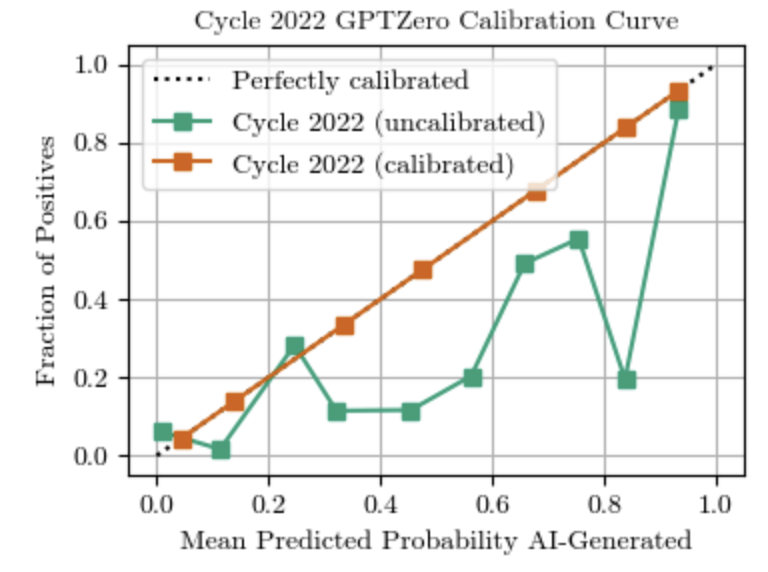
\includegraphics[width=0.4\textwidth]{figures/generative_ai/calibration.png}
    \caption{Calibration Curve of GPTZero's Predicted Probability AI-Generated, Cycle 2022}
    \label{fig:c2_calibration}
\end{figure}

With access to a large body of essays of known provenance ($15,149$ applicant-submitted Cycle 2022 essays and $5,002$ researcher-prompted ChatGPT-generated essays), we may use powerful calibration techniques comparing likelihood estimates to observed probabilities \cite{Zadrozny_Elkan_2002,Niculescu-Mizil_Caruana_2005}. Thus, we use isotonic calibration to calibrate GPTZero scores and produce $\widehat{P(AI)}$ \cite{Zadrozny_Elkan_2002}. We use this calibrated statistic in aggregate analyses and evaluate its utility according to its performance across all thresholds. I.e., we evaluate $\widehat{P(AI)}$ according to the area under its Receiver Operating Characteristic (ROC) curve (its ROC AUC score). We note that, in this case, a ROC AUC score of $0.5$ would indicate no discriminatory power, and a ROC AUC of $1.0$ would indicate perfect performance. We follow best practices in demanding an `acceptable' ROC AUC of at least $0.7$ \cite{Mandrekar_2010}.

\subsection{AI Detection In Lower-Stakes Decision-Making}
Finally, we are also interested in utilizing GPTZero outputs in lower-stakes decisions. This includes using these determinations to surface applicants who may require additional review or diligence, but extends also to determinations about an organisation's selection processes, pipeline, and outreach methods. Unlike in usage for automatic disqualification, this flag will only be used to draw additional selector attention to specific applications, and thus need not meet the $FPR \leq 0.02$ requirement. Instead, we focus on flagging application essays that are more likely to be AI-generated than not. That is, we use the threshold of $P(AI) \geq 0.5$ for this process. We opt to use this flag, rather than a raw probability, in analyses pertaining to an organisation's pipeline, as organisations often require more qualitative analysis of specific applications, and a binary indicator serves the secondary function of selecting these applications for us.

\section{Results}
\subsection{AI Detection In High-Stakes Decision-Making}\label{ssec:res_accuracy}
\subsubsection{The Veracity of AI Detection}
To determine how accurately we can identify AI-generated content, we compare the output statistic from our detector with actual knowledge of whether an essay was human- or computer-generated in Cycle 2022. We draw a ROC curve and report the area under that curve in Figure \ref{fig:c2_roc}. It does not matter here whether we use the calibrated or uncalibrated statistic, as the calibration process applies a monotonic transformation. The area under this ROC curve is an `outstanding' $0.91$, indicating good statistical power \cite{Mandrekar_2010}.

\begin{figure}[tbh]
    \centering
    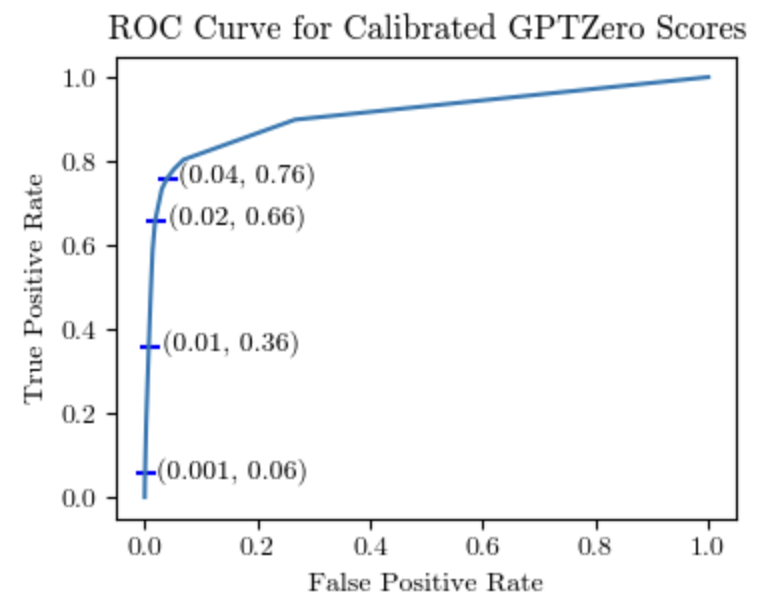
\includegraphics[width=0.4\textwidth]{figures/generative_ai/ROC.png}
    \caption{Receiver Operating Characteristic Curve of Calibrated GPTZero Scores, Cycle 2022}
    \label{fig:c2_roc}
\end{figure}

Despite good overall statistical power, GPTZero does not perform sufficiently well for the program to disqualify applicants on its basis alone. Section \ref{ssec:exp_accuracy} set a target of at least of $0.75$ TPR at $0.02$ FPR due to the program selecting only $2\%$ of completed applications. However, as Table \ref{tab:c2_tprs} shows (and as seen in Figure \ref{fig:c2_roc}), the threshold with a $2\%$ FPR identifies $66\%$ of AI-generated essays, leaving a third of such essays undetected and falling under our target of $0.75$ TPR.

\begin{table}[tbh]
   \centering
   \caption{Receiver Operating Characteristic AUC and Specificities, Cycle 2022}
   \label{tab:c2_tprs}
   \begin{tabular}{ l r }
       \toprule
       ROC AUC & $0.91$ \\
       TPR at $0.1\%$ FPR & $6\%$ \\
       TPR at $1\%$ FPR & $36\%$ \\
       TPR at $2\%$ FPR & $66\%$ \\
       TPR at $4\%$ FPR ($0.5$ Threshold) & $76\%$ \\
       \bottomrule\\
   \end{tabular}
\end{table}

\subsubsection{Heterogeneous Bias in AI Detection}
We next evaluate whether GPTZero is biased, on average, against genuine submissions from applicants with specific backgrounds. We conduct analyses of variance (ANOVAs) of the calibrated probability across gender and region categories in applicant-submitted essays from Cycle 2022 in Table \ref{tab:demo_anova}. As we know this data to be human-generated, this tests whether our detection method has heterogeneous false positive rates.

\begin{table}[htb]
    \centering
    \caption{Analysis of Variance for Calibrated Probability AI-Generated, Cycle 2022}
    \label{tab:demo_anova}
    \begin{tabular}{ l r r}
        \toprule
        Dimension & F Statistic & p Value \\
        \midrule
        Gender Identity & $41.4$ & $<0.01$ \\
        Region & $62.9$ & $<0.01$ \\
        \bottomrule\\
    \end{tabular}
\end{table}

\begin{table}[tbh]
    \centering
    \caption{Calibrated Probability AI-Generated and Inter-Cycle Changes by Applicant Demographics}
    \label{tab:demo_means}
    \begin{tabular}{ l r r r r r r}
        \toprule
        & \multicolumn{2}{c}{Cycle 2022} &  \multicolumn{2}{c}{Cycle 2023} & \multicolumn{2}{c}{Inter-Cycle T-Test} \\
        \cmidrule(lr){2-3} \cmidrule(lr){4-5} \cmidrule(lr){6-7}
        Demographic & Essays & $E(\widehat{P(AI)})$ & Essays & $E(\widehat{P(AI)})$ & t Score & p Value \\
        \midrule
        Male    & $6,475$ & $0.09$ & $11,080$ & $0.11$ & $8.63$ & $<0.01$ \\
        Female  & $8,710$ & $0.11$ & $13,380$ & $0.11$ & $-0.40$ & $0.69$ \\
        Other   & $176$   & $0.14$ & $355$    & $0.12$ & $-1.10$ & $0.27$ \\
        \midrule
        Caribbean               & $128$     & $0.17$ & $75$    & $0.15$ & $-0.47$ & $0.64$ \\
        ESEA     & $1,332$   & $0.13$ & $395$   & $0.13$ & $0.74$ & $0.46$ \\
        Five Eyes               & $522$     & $0.21$ & $1,865$ & $0.14$ & $-5.86$ & $<0.01$ \\
        Post-Soviet     & $85$      & $0.13$ & $705$   & $0.15$ & $0.59$ & $0.56$ \\
        South Asia     & $2,130$   & $0.08$ & $2,560$ & $0.09$ & $2.65$ & $0.01$ \\
        Latin America           & $709$     & $0.13$ & $2,855$ & $0.09$ & $-1.44$ & $0.15$ \\
        MENA   & $1,363$   & $0.11$ & $4,100$ & $0.12$ & $1.67$ & $0.09$ \\
        Subsahara      & $8,972$   & $0.09$ & $8,375$ & $0.09$ & $2.15$ & $0.03$ \\
        Other Europe            & $59$      & $0.20$ & $560$   & $0.12$ & $-2.75$ & $0.01$ \\
        Pacific Islands         & $5$       & $0.04$ & $0$      &  &  &  \\
        \midrule
        All         & $15,149$  & $0.10$ & $24,815$  & $0.11$ &  &  \\
        \bottomrule
    \end{tabular}
    % \begin{tablenotes}
    %     \small
    %     \item `Five Eyes' consists of Australia, Canada, New Zealand, the United Kingdom, and the United States.
    %     \item `MENA' stands for Middle East/North Africa.
    %     \item `ESEA' stands for East and Southeast Asia.
    %     \item $\widehat{E(P(AI))}$ is the mean estimated probability of essays being completely AI-generated.
    % \end{tablenotes}
\end{table}

Table \ref{tab:demo_anova} shows statistically significant variation across both dimensions in Cycle 2022. We therefore examine mean scores by gender identity and by countries of citizenship (grouped into larger categories). Column 3 of Table \ref{tab:demo_means} reports mean calibrated probabilities of being completely AI-generated for Cycle 2022 applicant submissions, which we know all predate ChatGPT. This shows that male applicants' essays receive lower estimates, on average, than applicants identifying as female or reporting some other gender category. While the magnitude of the difference is small, it raises the risk that using such scores in decision-making would bias outcomes against content genuinely created by women. Column 3 of Table \ref{tab:demo_means} also show genuinely human-generated applications from the Five Eyes – a group consisting of Australia, Canada, New Zealand, the United Kingdom, and the United States – get above average GTPZero scores. This is consistent with the fact that most large language models are trained primarily on texts from these countries, and may therefore align most closely with the style and lexical choices applicants from these countries use \cite{brown_language_2020}. However, as this bias appears to function in favor of non-native English speakers, it challenges previous work suggesting AI detectors are biased \textit{against} non-native English speakers \cite{liang_gpt_2023}.

\subsubsection{On Disqualifying Applicants via AI Detection}
We find here that no threshold meets our $FPR \leq 0.02$, $TPR \geq 0.75$ requirement for use in high-stakes decisions such as disqualifying candidates. Furthermore, we note that heterogeneous bias across a variety of demographic characteristics threaten to introduce biases into any process that uses this process to disqualify candidates. 

However, though we cannot meet the high bar of certainty required to disqualify a candidate, we may still be able to aggregate this information to yield valuable cohort-level insights, and may also use this information for lower-stakes decision-making (such as flagging a candidate for manual review).

\subsection{AI Detection in Aggregate Statistics}\label{ssec:res_statistics}
\subsubsection{The Analytic Utility of GPTZero}
Recall that the area under $\widehat{P(AI)}$'s ROC curve in Figure \ref{fig:c2_roc} is an `outstanding' $0.91$ (see: Table \ref{tab:c2_tprs}) \cite{mandrekar_receiver_2010}. This far exceeds our requirement of $0.80$ laid out in Section \ref{ssec:exp_statistics}, indicating that $\widehat{P(AI)}$ performs well at a variety of thresholds, and that use of this statistic in aggregate analysis will yield valuable results. 

We note as a caveat that our $\widehat{P(AI)}$ exhibits heterogeneous bias across demographic groups. Thus, analyses comparing GPTZero scores across different demographic subgroups risk conflating genuine difference in generative AI usage with measurement biases. We therefore focus primarily on analysing within-group changes in $\widehat{P(AI)}$.

\subsubsection{Applicants' Potential Use of AI-Generated Content}
We focus our subsequent analysis primarily on the potential use of generative AI by applicants in Cycle 2023. We note here that the mean probability of an essay being AI-generated within a corpus is exactly the expected proportion of AI-generated content within that corpus. Thus, we test for changes in mean $\widehat{P(AI)}$. Table \ref{tab:demo_means} presents mean $\widehat{P(AI)}$ for 2023 (column 3) and 2022 (column 5), as well as test statistics of whether there is a difference in means (columns 6 and 7).

\begin{table*}[tbh]
    \centering
    \caption{ANOVA for differences in GPTZero Detection Scores by Partners, Cycle 2023 }
    \label{tab:c3_partner_anova}
    \begin{tabular}{ l r r r r }
        \toprule
        \multicolumn{3}{c}{} & \multicolumn{2}{c}{ANOVA Results} \\
        \cmidrule(lr){4-5}
        Referring Partner & Essays & Share `AI-Generated' & F Statistc & p Value \\
        \midrule
        Partner A & $540$ & $0.041$ & $0.064$ & $0.80$ \\
        Partner B & $390$ & $0.044$ & $0.004$ & $0.95$ \\
        Partner C & $325$ & $0.049$ & $0.320$ & $0.57$ \\
        Partner D & $315$ & $0.029$ & $1.599$ & $0.21$ \\
        Partner E & $235$ & $0.064$ & $2.526$ & $0.11$ \\
        Partner F & $205$ & $0.039$ & $0.076$ & $0.78$ \\
        Partner G & $170$ & $0.047$ & $0.071$ & $0.79$ \\
        Partner H & $150$ & $0.027$ & $0.970$ & $0.33$ \\
        Partner I & $150$ & $0.007$ & $4.829$ & $0.03$ \\
        Partner J & $135$ & $0.022$ & $1.415$ & $0.23$ \\% suppressing to save space
        \midrule
        All Submissions & $24,815$ & $0.040$ & \\
        \bottomrule
    \end{tabular}
    % \begin{tablenotes}
    %     \small
    %     \item Share `AI-Generated' is the share of essays identified as more likely to be AI-generated than not.
    %     \item 
    % \end{tablenotes}
\end{table*}

We find statistically significant increases in the $\widehat{P(AI)}$ for only two overlapping subgroups: male applicants and applicants from the Indian subcontinent. In both cases the magnitude of the increase is small, suggesting that at least in Cycle 2023, the use of generative AI was limited. However, other findings preclude interpreting this change as a direct measure of increased generative AI use. In two regions, the Five Eyes and Europe (excluding the United Kingdom and former Soviet Union), we found a statistically significant decrease in the calibrated estimated probability that essays were completely AI generated. Since we can assume very few (if any) applicants in Cycle 2022 had access to generative AI, this cannot be interpreted as a decrease in AI use. It may instead be that both regions' high average scores in 2022 were a fluke of the cohort, and that these regions reverted to the mean in 2023. Alternatively, it is possible that, in these regions, Cycle 2023 applicants used AI detection tools to ensure that their content would not be flagged by our detector (although this would require such detector usage to offset any actual generative AI use) \cite{gptzero_gptzero_2023}. In either case, this analysis surfaces interesting discrepancies demanding further interrogation in future application cycles. 

\subsection{AI Detection In Lower-Stakes Decision-Making}
\subsubsection{Flagging Applicants Likely to Have Used Generative AI}\label{ssec:flags}
In Cycle 2023 decision-making, our partner program used GPTZero's AI detection to ``flag'' applicants that we believe are likely to be AI-generated. As previously mentioned, we do not have sufficient confidence in the statistical power of fairness of any determination we could make to disqualify applicants for possible generative AI usage. We have set a high bar for such confidence. However, we might still use these flags to direct human reviews of application essays, or to evaluate our application pipeline.

For this process, we use a cutoff of $0.5$ on our calibrated predictor, meaning that essays flagged as `AI-Generated' are more likely than not to be so ($\widehat{P(AI)} \geq 0.5$). This threshold is shown in Table \ref{tab:c2_tprs} with a true positive rate of $76\%$ and a false positive rate of $4\%$.

In practice, the program used these flags throughout Cycle 2023 to direct the attention of human reviewers towards essays that were likely to be AI-generated. We note that the program did not ban the usage of generative AI, so these applicants were not penalised for these determinations. However, generative AI's tendencies towards plagiarism are well-documented, and the program did devote additional attention towards catching plagiarism in flagged applicants \cite{dehouche_plagiarism_2021}.

\subsubsection{Evaluating Partners with AI Detection}
Talent identification programs are perennially interested in reaching talent across their target demographic. Our partner program employs an outreach strategy of cultivating relationships with `referring partners', i.e., organisations that encourage and support applicants. Relevant applicants are attributed to referring partners based on the custom links applicants use to reach the program's website, as well as questions in the application form about how applicants learned of the program.

As these partnerships form a large portion of the program's outreach, the program regularly evaluates the utility of this approach. As part of this evaluation, the program evaluates the likelihood of irregular generative AI usage in the essays associated with the program's referring partners. Evidence that any of the referring partners used generative AI to create large volumes of applications would warrant further investigation before continuing said partnerships.

For this evaluation, we associate flagged essays with the appropriate referring partners. For the purposes of this paper and to preserve the program's anonymity, we have limited this analysis to the partners with the most essays and have hidden individual partners' identities. We then conduct an ANOVA to test for variations in the frequency of flagged essays by partner. Table \ref{tab:c3_partner_anova} shows the results of this ANOVA.

Here, only one of the partners studied was associated with essays identified as AI-generated at a rate meaningfully different from the overall pool. However, the partner in question, Partner I, was actually associated with fewer essays than average identified as AI-generated. This may be driven by the (Africa-based) partner working primarily with demographics identified in Cycle 2022 analyses as naturally having below-average calibrated scores. Overall, the program found no evidence of generative AI usage associated with any particular partner, which served as an important step in validating program involvement with these partners.

\section{Discussion}\label{sec:conc}
Our natural experiment on Cycle 2022 data enjoyed optimal conditions for AI detection; the synthetic essays were not paraphrased or edited, and all of the human-written essays were real submissions to the program. Despite this, at sensitivity levels comparable to acceptance rates into selective programs, we do not achieve high specificity. Thus, we conclude that the program should not use this technology in making high-stakes decisions such as disqualifying candidates. Furthermore, we find heterogeneous biases in our detection of AI essays. We do, however, see good overall statistical power. Therefore, we find utility in using AI detection for aggregate analyses, so long as these analyses account for the risk of heterogeneous biases. We demonstrate one such analysis on data supplied by the program: examining the potential scale of AI usage by demographic group. Finally, we note that organisations may still use determinations in making lower-stakes decisions such as the direction of additional selector scrutiny and post-hoc evaluation of application pathways. We conclude that organisations looking to assess the use of generative AI in essays they receive have an opportunity to do so with GPTZero or other AI detection tools.

This analysis is limited in scope to only one method for AI generation and one method for identification of that generation. Thus, our present results are limited to these methods. One avenue for future analyses include using other methods of essay generation and AI detection and seeking out differential performance on essays in response to particular prompts. In particular, we intend further work to focus on understanding the effect of paraphrasing software on our results, as the paraphrasing of generative AI outputs has been shown to render them less detectable \cite{mitchell_detectgpt_2023,kalpesh_krishna_paraphrasing_2023}.

Furthermore, the work with our partner program is longitudinal and ongoing, and our partner program is presently administering application Cycle 2024. We intend to incorporate the 2024 application cycle into our analyses going forward, and to further extend this with subsequent application cycles.